% ============================================================
\chapter{Spectral Analysis}
\label{ch:spectrale}
% ============================================================

\section{Motivating Example}
A climate signal contains cycles of different periods (daily, annual, El Ni\~no). Spectral analysis decomposes the total variance by frequency, revealing hidden periodicities.

\section{Spectral Density}\index{spectral density}

\begin{definition}[Power Spectral Density]
If $\sum_{h=-\infty}^{\infty}|\gamma(h)|<\infty$, the \textbf{spectral density} of $(X_t)$ is:
\[
f(\omega) = \frac{1}{2\pi}\sum_{h=-\infty}^{\infty}\gamma(h)\,e^{-i\omega h}, \quad \omega\in[-\pi,\pi].
\]
This is the Fourier transform of the autocovariance function.
\end{definition}

\begin{theorem}[Properties of $f$]
\begin{enumerate}
\item $f(\omega)\geq 0$ for all $\omega$.
\item $f$ is even: $f(\omega)=f(-\omega)$.
\item Inversion formula: $\gamma(h) = \int_{-\pi}^{\pi}f(\omega)\,e^{i\omega h}\,d\omega$.
\item $\gamma(0) = \Var(X_t) = \int_{-\pi}^{\pi}f(\omega)\,d\omega$ (Parseval's theorem).
\end{enumerate}
\end{theorem}

\begin{proof}[Sketch of (1)]
By Herglotz's theorem, $\gamma$ is positive semi-definite. Hence $f(\omega)=\frac{1}{2\pi}\sum\gamma(h)e^{-i\omega h}\geq 0$ (as a limit of positive quadratic forms).
\end{proof}

\section{Spectra of Classical Processes}

\begin{theorem}[Spectrum of an ARMA$(p,q)$]
\[
f(\omega) = \frac{\sigma^2}{2\pi}\,\frac{|\theta(e^{-i\omega})|^2}{|\phi(e^{-i\omega})|^2}.
\]
\end{theorem}

\begin{example}[Spectrum of an AR(1)]
$\phi(z)=1-\phi z$:
\[
f(\omega) = \frac{\sigma^2}{2\pi}\,\frac{1}{|1-\phi e^{-i\omega}|^2} = \frac{\sigma^2}{2\pi(1-2\phi\cos\omega+\phi^2)}.
\]
If $\phi>0$: peak at $\omega=0$ (dominant low frequencies). If $\phi<0$: peak at $\omega=\pi$.
\end{example}

\begin{center}
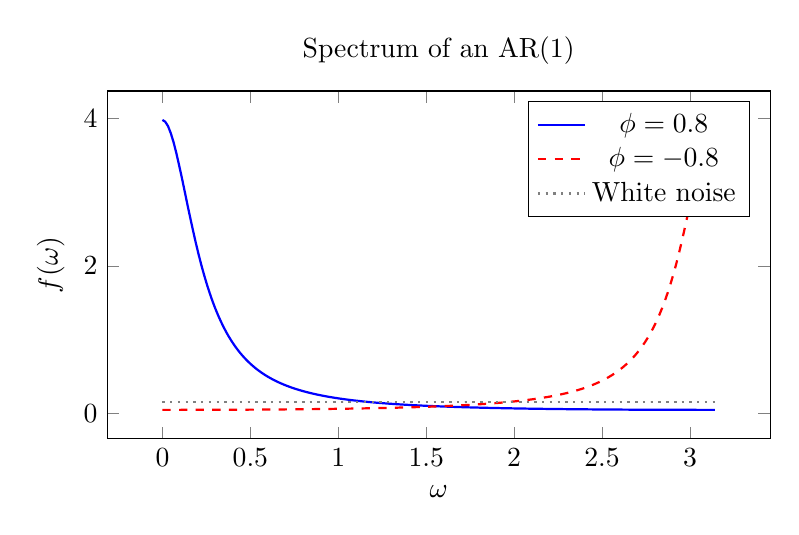
\begin{tikzpicture}
\begin{axis}[
  width=10cm, height=6cm,
  xlabel={$\omega$}, ylabel={$f(\omega)$},
  title={Spectrum of an AR(1)},
  domain=0:3.14159, samples=200,
  legend pos=north east
]
\addplot[thick,blue] {1/(2*3.14159*(1-2*0.8*cos(deg(x))+0.64))};
\addlegendentry{$\phi=0.8$}
\addplot[thick,red,dashed] {1/(2*3.14159*(1+2*0.8*cos(deg(x))+0.64))};
\addlegendentry{$\phi=-0.8$}
\addplot[thick,gray,dotted] {1/(2*3.14159)};
\addlegendentry{White noise}
\end{axis}
\end{tikzpicture}
\end{center}

\section{Periodogram}\index{periodogram}

\begin{definition}[Periodogram]
The naive estimator of $f(\omega)$:
\[
I_n(\omega) = \frac{1}{2\pi n}\left|\sum_{t=1}^n X_t\,e^{-i\omega t}\right|^2.
\]
\end{definition}

\begin{theorem}[Properties of the Periodogram]
\begin{enumerate}
\item $\E[I_n(\omega_j)]\to f(\omega_j)$ at the Fourier frequencies $\omega_j=2\pi j/n$.
\item $I_n(\omega_j)$ is an \textbf{inconsistent} estimator: $\Var(I_n(\omega_j))\not\to 0$.
\item At Fourier frequencies: $I_n(\omega_j)/f(\omega_j)\stackrel{\text{approx}}{\sim}\chi^2(2)/2$.
\end{enumerate}
\end{theorem}

\begin{warning}
The raw periodogram is very erratic. It must be smoothed to obtain a consistent estimator.
\end{warning}

\section{Spectral Estimation}\index{spectral estimation}

\subsection{Spectral Window (Smoothing)}

\begin{definition}[Smoothed Periodogram]
\[
\hat{f}(\omega) = \sum_{|h|\leq M} w(h)\,\hat{\gamma}(h)\,e^{-i\omega h},
\]
where $w$ is a \textbf{window} (Bartlett, Parzen, Tukey, etc.) and $M$ is the \textbf{bandwidth}.
\end{definition}

\subsection{Parametric Method}

Estimate an AR$(p)$ model by Yule--Walker or Burg, then use the theoretical spectrum $\hat{f}(\omega)=\frac{\hat\sigma^2}{2\pi|\hat\phi(e^{-i\omega})|^2}$.

\section{Implementation}

\begin{codeblock}[title=\textbf{Python}]
\begin{minted}{python}
import numpy as np
import matplotlib.pyplot as plt
from scipy.signal import periodogram, welch

# Simuler un AR(2) avec pic spectral
np.random.seed(42)
n = 1024
eps = np.random.normal(0, 1, n)
x = np.zeros(n)
phi1, phi2 = 1.5, -0.85  # racines complexes => pic
for t in range(2, n):
    x[t] = phi1*x[t-1] + phi2*x[t-2] + eps[t]

# Périodogramme brut
freq_p, Pxx_p = periodogram(x, fs=1, scaling='density')

# Périodogramme lissé (Welch)
freq_w, Pxx_w = welch(x, fs=1, nperseg=256, scaling='density')

fig, axes = plt.subplots(1, 2, figsize=(14, 5))
axes[0].semilogy(freq_p, Pxx_p, lw=0.5)
axes[0].set_title('Périodogramme brut')
axes[0].set_xlabel('Fréquence')

axes[1].semilogy(freq_w, Pxx_w, lw=1.5, color='red')
axes[1].set_title('Périodogramme lissé (Welch)')
axes[1].set_xlabel('Fréquence')

plt.tight_layout()
plt.savefig('ch07_spectral.pdf')
plt.show()

# Spectre théorique AR(2)
omega = np.linspace(0.01, np.pi, 500)
phi_z = 1 - phi1*np.exp(-1j*omega) - phi2*np.exp(-2j*omega)
f_theo = 1 / (2*np.pi * np.abs(phi_z)**2)

plt.figure(figsize=(8, 4))
plt.plot(omega, f_theo, 'b-', label='Théorique')
plt.title('Spectre théorique AR(2)')
plt.xlabel('$\\omega$'); plt.ylabel('$f(\\omega)$')
plt.legend()
plt.savefig('ch07_spectral_theo.pdf')
plt.show()
\end{minted}
\end{codeblock}

\section{Exercises}

\begin{exercise}[$\star$]
Compute the spectral density of an MA(1): $X_t=\eps_t+\theta\eps_{t-1}$.
\end{exercise}

\begin{exercise}[$\star\star$]
Show that the periodogram can be written as $I_n(\omega)=\sum_{|h|<n}\hat\gamma(h)e^{-i\omega h}/(2\pi)$.
\end{exercise}

\begin{exercise}[$\star\star$]
Prove that for a Gaussian white noise, $2nI_n(\omega_j)/\sigma^2\sim\chi^2(2)$ at nonzero Fourier frequencies.
\end{exercise}

\begin{exercise}[$\star\star\star$ -- Project]
Analyze the spectrum of daily temperatures in Paris over 50 years. Identify the peaks corresponding to the annual, semi-annual, and weekly cycles.
\end{exercise}

\begin{keyformulas}
\begin{align*}
f(\omega) &= \frac{1}{2\pi}\sum_{h}\gamma(h)e^{-i\omega h}, \quad \gamma(h)=\int_{-\pi}^{\pi}f(\omega)e^{i\omega h}d\omega \\
f_{\text{ARMA}}(\omega) &= \frac{\sigma^2}{2\pi}\frac{|\theta(e^{-i\omega})|^2}{|\phi(e^{-i\omega})|^2} \\
I_n(\omega) &= \frac{1}{2\pi n}\left|\sum_{t=1}^n X_t e^{-i\omega t}\right|^2
\end{align*}
\end{keyformulas}
